\clearpage
\begin{center}
\huge{\textbf{Opinion Dynamics on Social Network}} 
\end{center}
\newpage
\newcommand{\twopartdef}[4]
{
	\left\{
		\begin{array}{ll}
			#1 & \mbox{if } #2 \\
			#3 & \mbox{if } #4 
		\end{array}
	\right.
}
\section*{Introduction}
Opinion Dynamics means how opinions change with time in a social network. Many social networks that we see nowadays are characterized by opinion. Here opinion means for a given node (say user in Twitter or Reddit) and a given topic (say release of an upcoming movie) we want to study how the opinions vary with time especially say before and after some specific event (like the release of the movie). Also all these social networks have an underlying network between the nodes (like friend and follower in Twitter and friends in Facebook) and opinions usually flow among these networks (like say we get influenced by the review of a movie from a friend of us and we also get the same opinion without even seeing the movie). Now in social networks nodes have many such influence but if we dont have the information about how a particular user likes content of another particular influence then they are just binary - influences or not. But in real social network we have preference of opinion among our friends and also this may be both positive and negative (like if we already know that our movie choices does not match with our friends then our opinion on a particular movie is likely to be opposite).
\\
So in this work we take input a network of nodes (with a directed follower relationship) a set of opinions of the particular user on a particular topic in a time window. Now given this data we try to qunatize the influences between the nodes. Also another questions that we may ask are say given just the opinion values can we infer the influence network (completely unsupervised) and also after quantization can we use our model to predict future opinion sentiments of the nodes
\\
So typical usage scenerio can be in Election poll forcasting where we have the opinion values before election and we can predict the results. This can also be used while the campaign is going on to test whether the social media is coming on our side or not. It also has vast application in E-commerce. For example if an ecommerce is trying to launch two products together say Galaxy S6 and Iphone 6 and the ecommerce firms can gather the social data and infer which product is going to lead and restock accordingly and this is possible because we often get influenced by the transactions and reviews made by our peers. Also another optimistic usage can be 'review manipulation'. For example if we want to sell more IPhones then given the model we set our target opinion and use our model to find an initial condition which might lead to this final state. Once we find the initial conditions we can incentivize nodes according to the finding and if it behaves according to our learned model then its a huge gain for such ecommerce firms.
\section*{Formal Problem Definition}
We have a directed binary influence matrix $N$ i.e. if $N(x,y) = 1 \Longleftrightarrow x $is following $y$ and $N(x,y) = 0 \Longleftrightarrow x$ is not following $y$. Also we have a set of opinion values for each node in a time window. So we will divide the opinions in two sets by fixing a time separator. Opinion before the separator are in 'training' and after that are in 'test'. So using the training data we will learn the quantified Influence Matrix $A$ and will try to predict opinions in the 'training' set.
\section*{The Voter Model}
Many models have been proposed on how opinions vary over time on a social network. One such particular model is Voter Model which is simple to describe. Steps are described in Figure~\ref{fig:voter_model}. It consists of the following simple steps - (i) pick a random node (a voter),(ii) the voter adopts the state of a random neighbor.

\begin{figure}
\centering
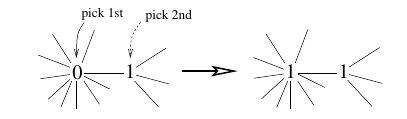
\includegraphics[width=\textwidth,height=\textheight,keepaspectratio]{opinion_dynamics/images/voter_model.png}
\caption{Opinion Dynamics in Voter Model}
\label{fig:voter_model}
\end{figure}
\section*{The proposed Model}
Now suppose in the train window for node $x$ we have the set of opinions $S_{x} = \{(O_{i},t_{i})|1 \leq i \leq k\}$. Now using voter model for every node we want to maximize $P(S_{x}|A)$. Now to effectively use voter model need to define the following quantities. Now we define $n_{t}$ as the opinion vector at time instance $t$. Now in real social networks nodes dont advertise their opinion at every timestamp. So we also define $n_{t-}$ as the opinion vector of the nodes strictly before the time $t$. We also define $n_{t,x}$ in the following manner,
\begin{equation}
n_{t,x} (y) = \twopartdef {n_{t-} (y)} {x \neq y} {1-{n_{t-} (y)}} {x = y}
\end{equation}
as our opinion values are discrete and we model them as $1$ or $0$ so negation with $1$ just complements the opinion. Now from the voter model we know that the Probability that a paricular node will change in a given a timestamp is nothing but
\begin{equation}
P(n_{t-} \rightarrow n_{t,x}) = \displaystyle\sum_{y} \frac{N_{x,y}}{Nk_{x}} \xi (x,y,t)
\end{equation}
where $k_{x}$ is the number of influences of the node $x$ if we assume a complete uniform voter model. Ansd the $\xi(x,y,t)$ is an indicator function which is defined as follows,
\begin{equation}
\xi(x,y,t) = \twopartdef {1} {n_{t-}(x) \neq n_{t-}(y)} {0} {n_{t-}(x) = n_{t-}(y)}
\end{equation}
\section*{Optimization Problem formation with Maximum Likelihood Estimation}
So in our proposed framework to come up with a MLE expression interms of $A$ we can use 
\begin{equation}
P(n_{t-} \rightarrow n_{t,x}) = \displaystyle\sum_{y} \frac{A_{x,y}}{N} \xi (x,y,t)
\end{equation}
where $\displaystyle\sum_{y} A_{xy}= 1$. Also note that we are only constrained by the $x$th row of A while while solving for $x$ and those parameters are in no other MLE as our graph is directed. So we can solve for each of the nodes separately and though this would take up a huge time but it is scalable as each of the opimization problems are tractable and all of them can done parallely accross distributed systems. Also from this we can say $P($node x does not flip at time t$) = 1 - P(n_{t-} \rightarrow n_{t,x}) = 1 - \displaystyle\sum_{y} \frac{A_{x,y}}{N} \xi (x,y,t)$. Using this definitions we can write $P(S_x|A) = P(n_{t_{i}}(x) = O_{t_{i}}(x),\forall t_i, 0 \leq i \leq k|A)$, where $O_{t_{i}}(x)$ is the observed opinion of node $x$ at time instant $t_i$. Hence\\
$P(S_x|A) \propto \displaystyle\prod_{i}^{k} P(n_{t_1}(x) = O_{t_i}(x)|A,n_{t-})P(n_{t_0}|A)$\\
$ \propto \displaystyle\prod_{i}^{k} P(n_{t_1}(x) = O_{t_i}(x)|A,n_{t-})$\\
$ = \displaystyle\prod_{i=1}^{k}(1 - \displaystyle\sum_{y} \frac{A_{x,y}}{N} \xi (x,y,t_i))^{I(n_{t_i}(x) = n_{t_i -}(x))}\displaystyle\prod_{i=1}^{k}(\displaystyle\sum_{y} \frac{A_{x,y}}{N} \xi (x,y,t_i))^{I(n_{t_i}(x) \neq n_{t_i -}(x))}$
\\
Now by taking logarithm on both sides we find
\\ $L = ln(P(S_{x}|G)) \propto \displaystyle\sum_{i=1}^{k}I(n_{t_i}(x) = n_{t_i -}(x))ln(1 - \displaystyle\sum_{y} \frac{A_{x,y}}{N} \xi (x,y,t_i)) + \displaystyle\sum_{i=1}^{k}I(n_{t_i}(x) \neq n_{t_i -}(x))ln(\displaystyle\sum_{y} \frac{A_{x,y}}{N} \xi (x,y,t_i))$.
\\
So our optimization problem is given maximize $L$ given $\displaystyle\sum_{y} A_{xy}= 1$.
\section*{Concave Maximization}
Here we will show that our problem is concave maximization problem. Basically $L$ is the summation of a log-linear function. Now for a function $f$ to be concave we must have $Z^{T}\nabla^{2}fZ \leq 0 \forall Z$.Also if $Z^{T}\nabla^{2}f_{1}Z \leq 0 \forall Z$ and $Z^{T}\nabla^{2}f_{2}Z \leq 0 \forall Z$, then $Z^{T}\nabla^{2}(f_{1}+f_{2})Z \leq 0 \forall Z$. So if we can prove the log-linear function $f = ln(\displaystyle\sum_{i}a_{i}x_{i} + c)$ is concave for $a_i,c \in \Re$ then we are done. Let $M = \displaystyle\sum_{i}a_{i}x_{i} + c$.
clearly $\nabla f (i) = \frac{a_i}{M}$
Also it is easy to show that $\nabla^2 f (i,j) = -\frac{a_ia_j}{M^2}$. Now if we define $D = [a_1,a_2,...,a_n]^T$. Then We can write $\nabla^2 f = \frac{1}{M^2} DD^T$. So for $Z \in \Re^n$ we have $Z^{T}\nabla^{2}fZ = -\frac{1}{M^2} (Z^TA)(Z^TA)^T \leq 0$. Hence the given optimization problem is a concave maximization and it can be easily solved numerically.
\section*{Implementation}
Now our optimization problem can be solved with gradient ascent, there are better methods. So this algorithm is implemented in mosek toolbox. For some experiments we used the given dataset, but we also developed modules to gather tweet stream from Twitter and extract friend follower information from Twitter. We also generated modules to generate synthetic data. We had to do many experiments by varying the time window that separates the train and test set and we also automated that. Now using the apis provided by the mosek api we developed modules to solve the maximum likelihood problems. For testing part, after learning the influence values we ran stochastic simulation on the test data and computed average output. We define accuracy as the overall fraction of opinion matches accross all the nodes in a particular simulation and we report the average one for several simulation with a particular time window.
\section*{Experimental Results}
In Figure~\ref{fig:Reddit_plot} we show how the accuracy varies accoring to the movement of the time window. In Figure~\ref{fig:Twitter_plot} we show it for the same. It seems that if we incrase the training data then the accuracy of our model increases in case of Reddit. But we don't find any recognizable trend in the Twitter Dataset. Which implies our model is not working on the Twitter dataset. This requires further examination.
\begin{figure}
\centering
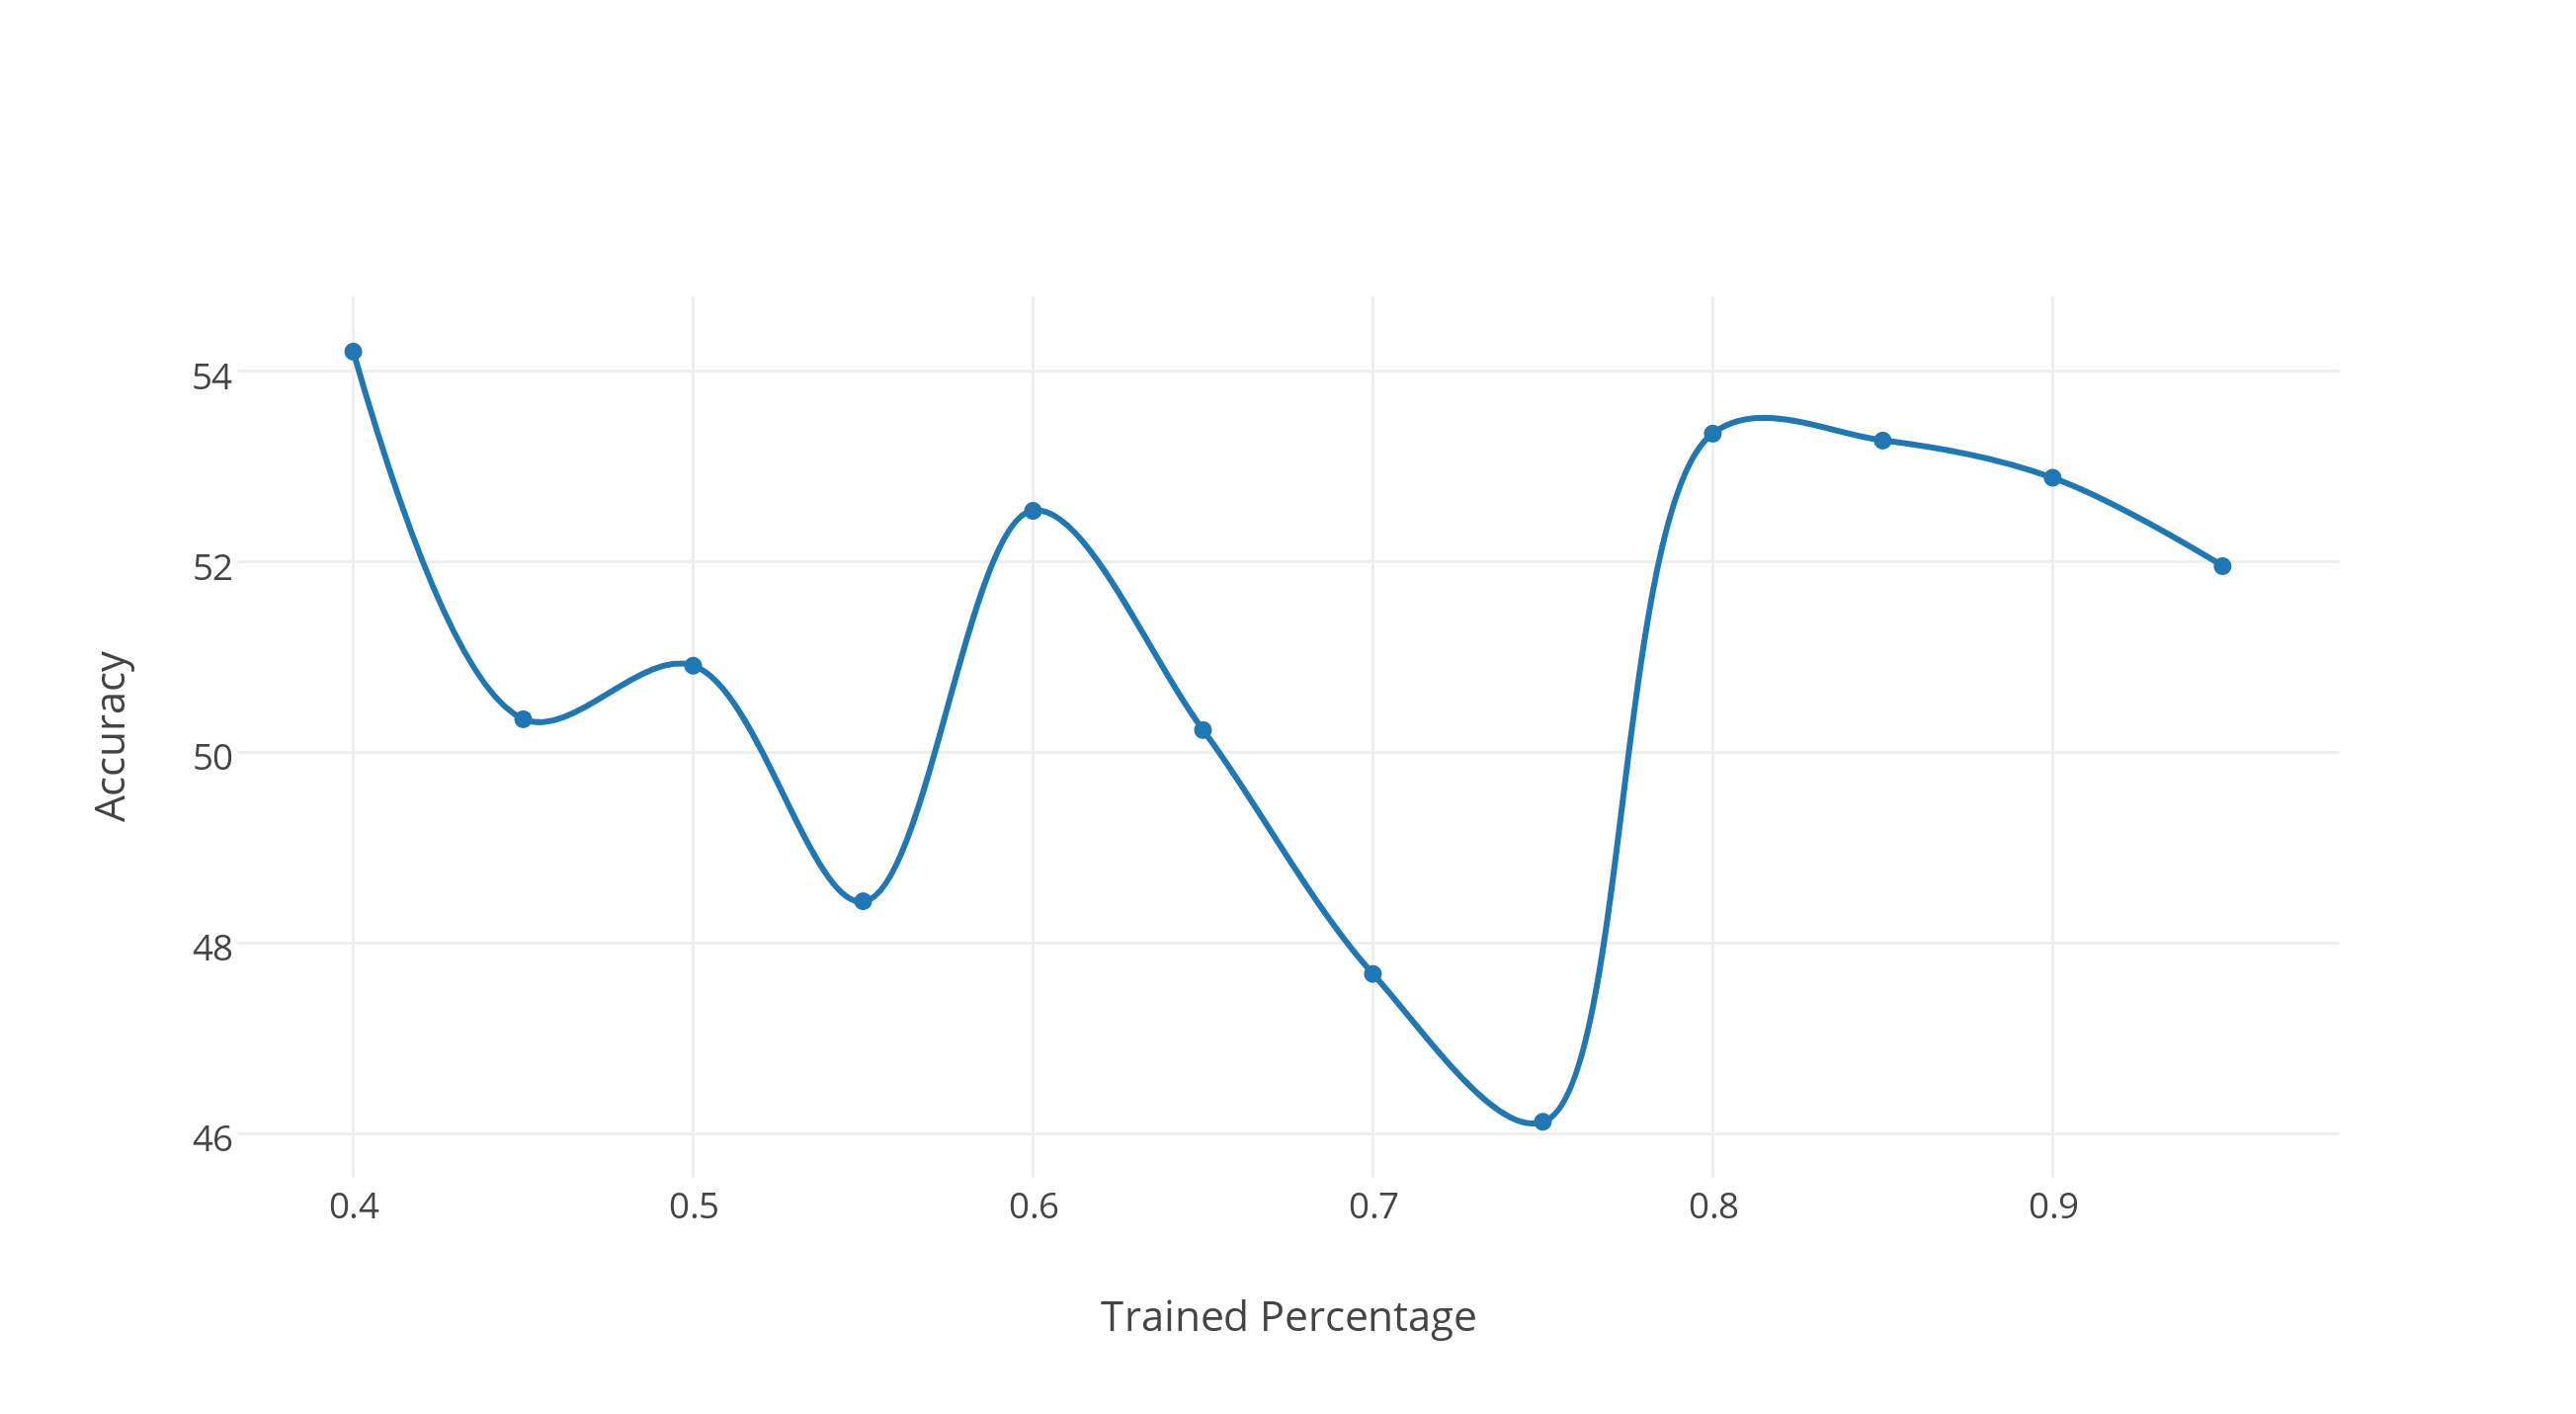
\includegraphics[width=\textwidth,height=\textheight,keepaspectratio]{opinion_dynamics/images/Twitter_plot.png}
\caption{Effect of time window variation on Twitter}
\label{fig:Twitter_plot}
\end{figure}
\begin{figure}
\centering
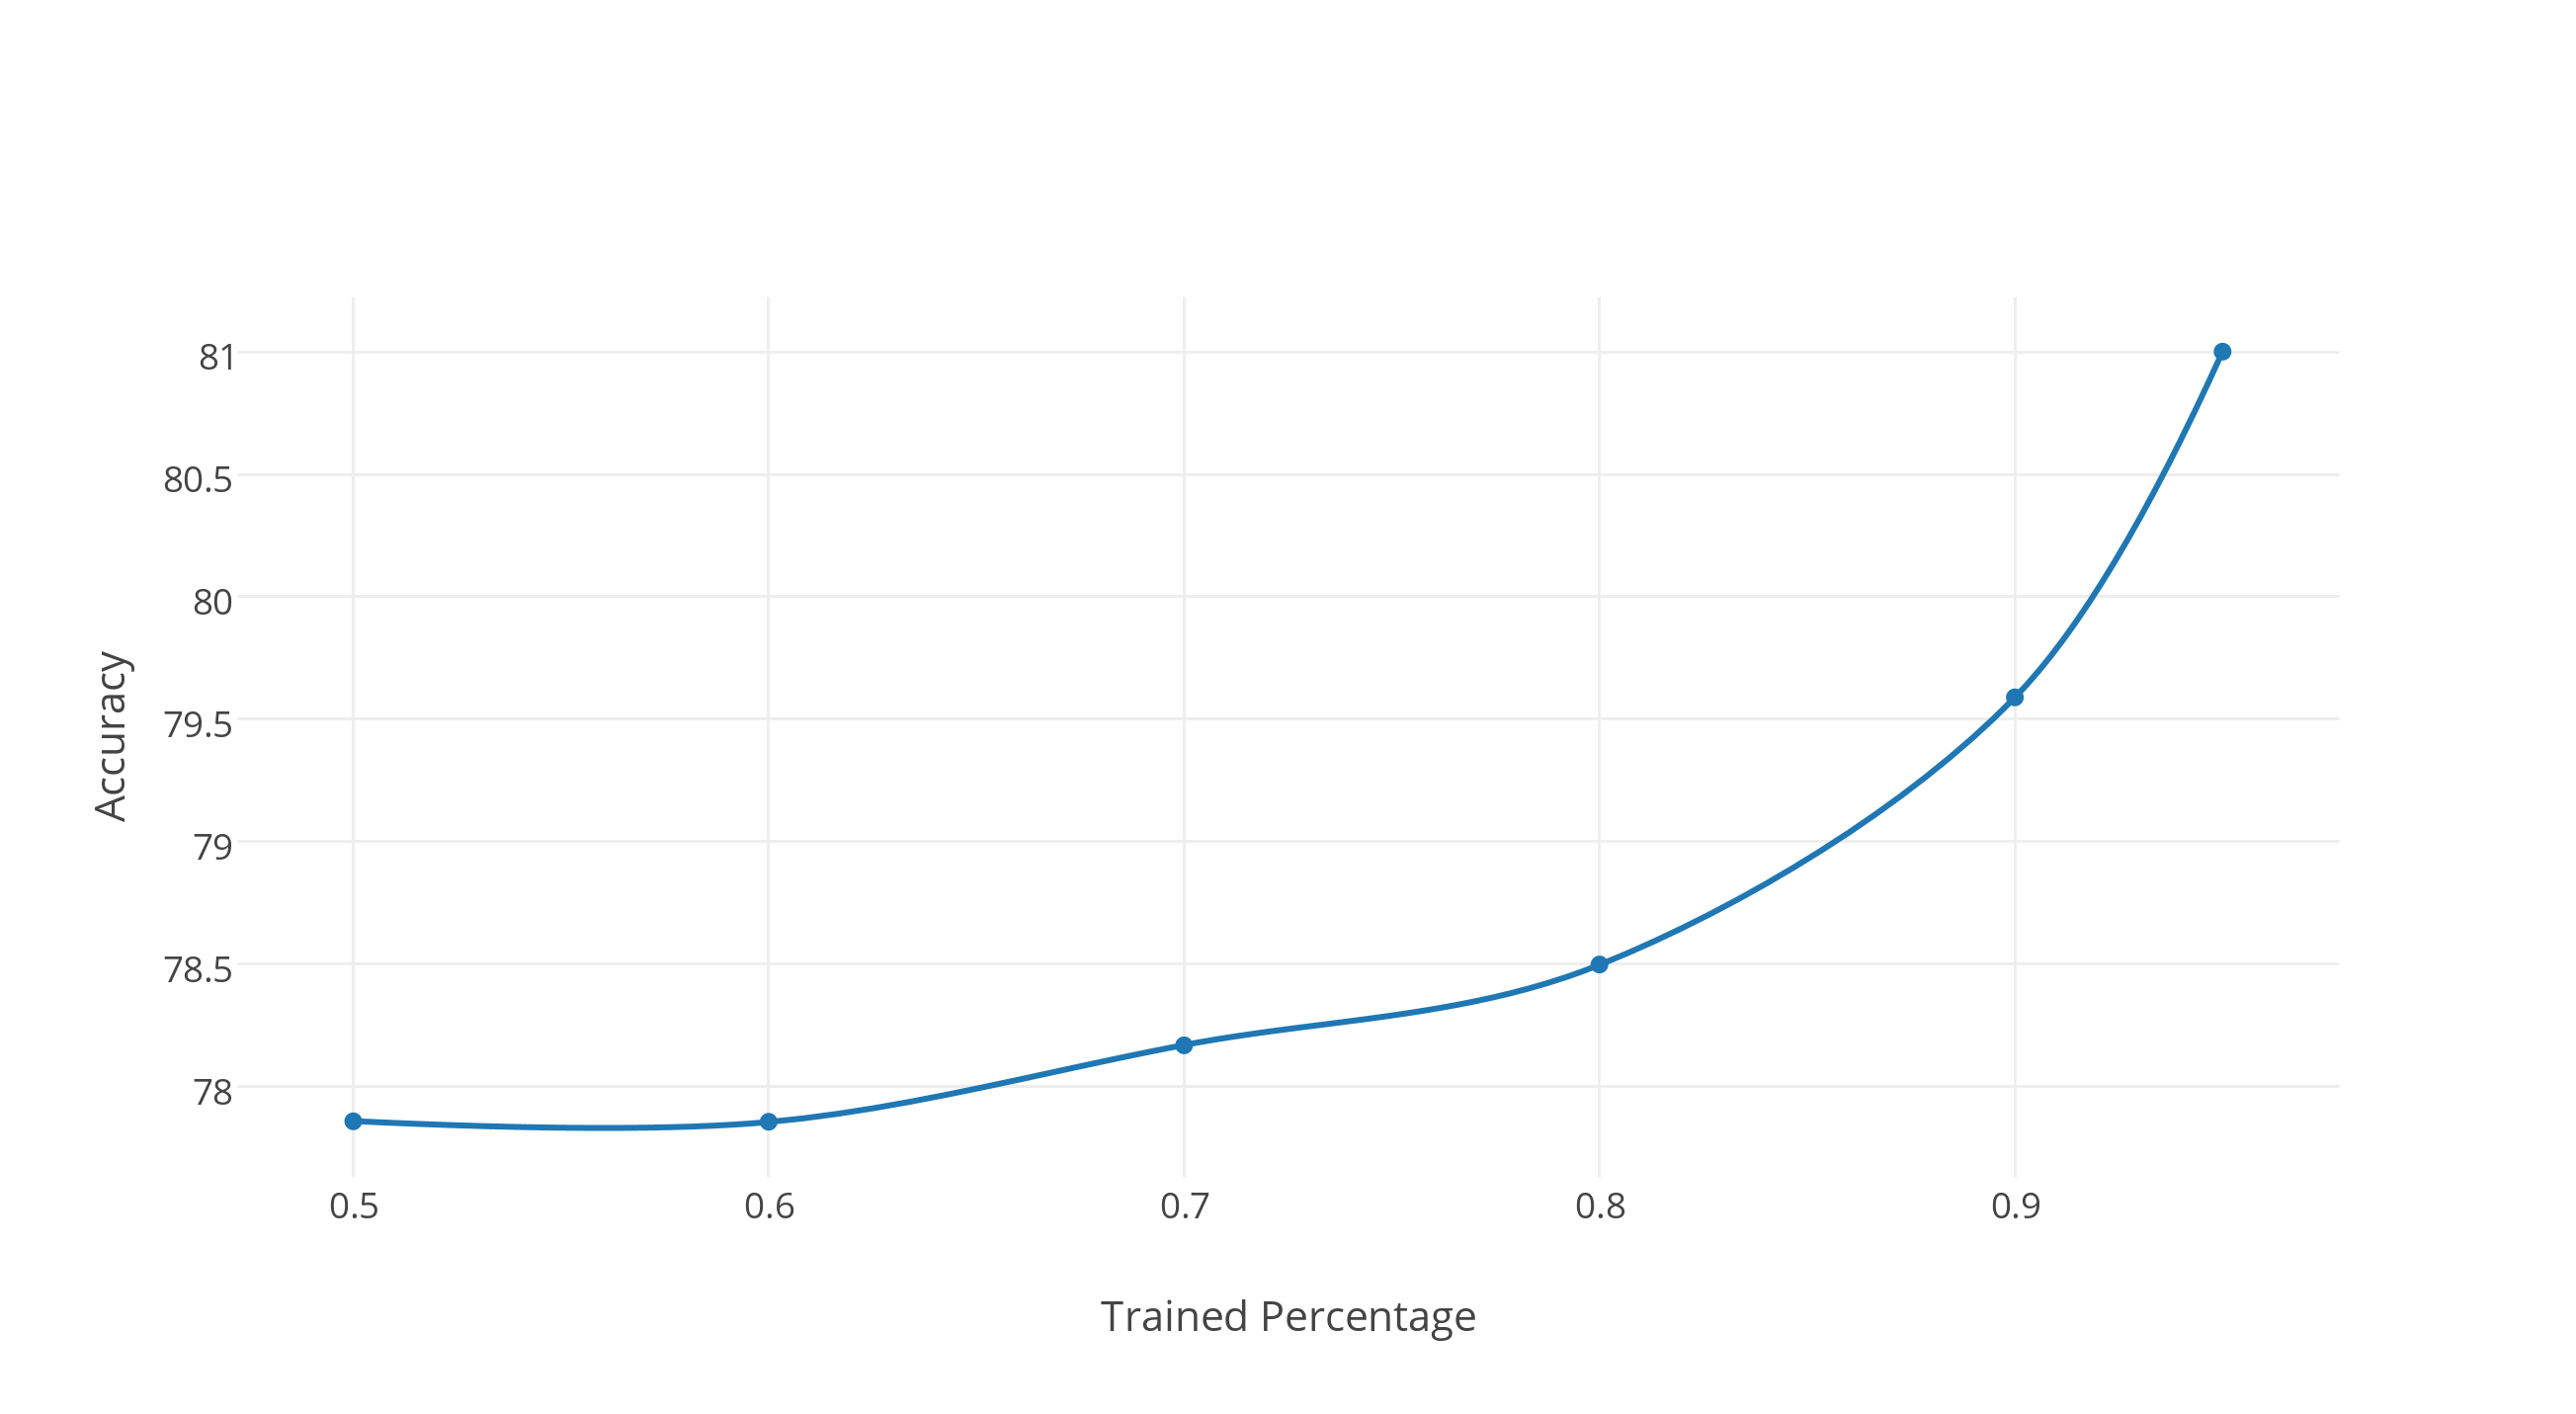
\includegraphics[width=\textwidth,height=\textheight,keepaspectratio]{opinion_dynamics/images/Reddit_plot.png}
\caption{Effect of time window variation on Reddit}

\label{fig:Reddit_plot}
\end{figure}
\section*{Drawbacks of the model}
Now there may be various drawbacks in the model. One thing we observed that though we get good accuracy in Reddit dataset, the model that we generate is too much sparse unlike a real network. Also as we showed that the optimization problem is a concave maximization, but its not strictly concave one. So there may be various solutions given a test data and we might not get always lucky to pick the model that gives the best test accuracy.
\section*{Towards a better model}